\documentclass[12pt]{article}

\usepackage{graphicx}
\graphicspath{{../Fichier_Image}}

\title{Hypothèse 1.(a) Taille couloirs principaux}
\author{Thibault Clodion}

\begin{document}

\maketitle % Permet d'afficher le titre, l'author etc

\underline{Hypothèse :} La taille des couloirs menant aux portes de sorties (juste devant)
doit être la même que celle de la porte de sortie
\newline\newline
\underline{Expérience :} Je vais repartir de la simulation n°1 (par facilité et pour tester avec des grands flux) et je vais proposer un couloir principal de taille 80cm, 1m, 1m25, 1m50, 2m
\newline\newline

1.(a) Couloir Principal 80cm :
\newline\newline
Temps moyen de dernière sortie : 32.70 s
\newline
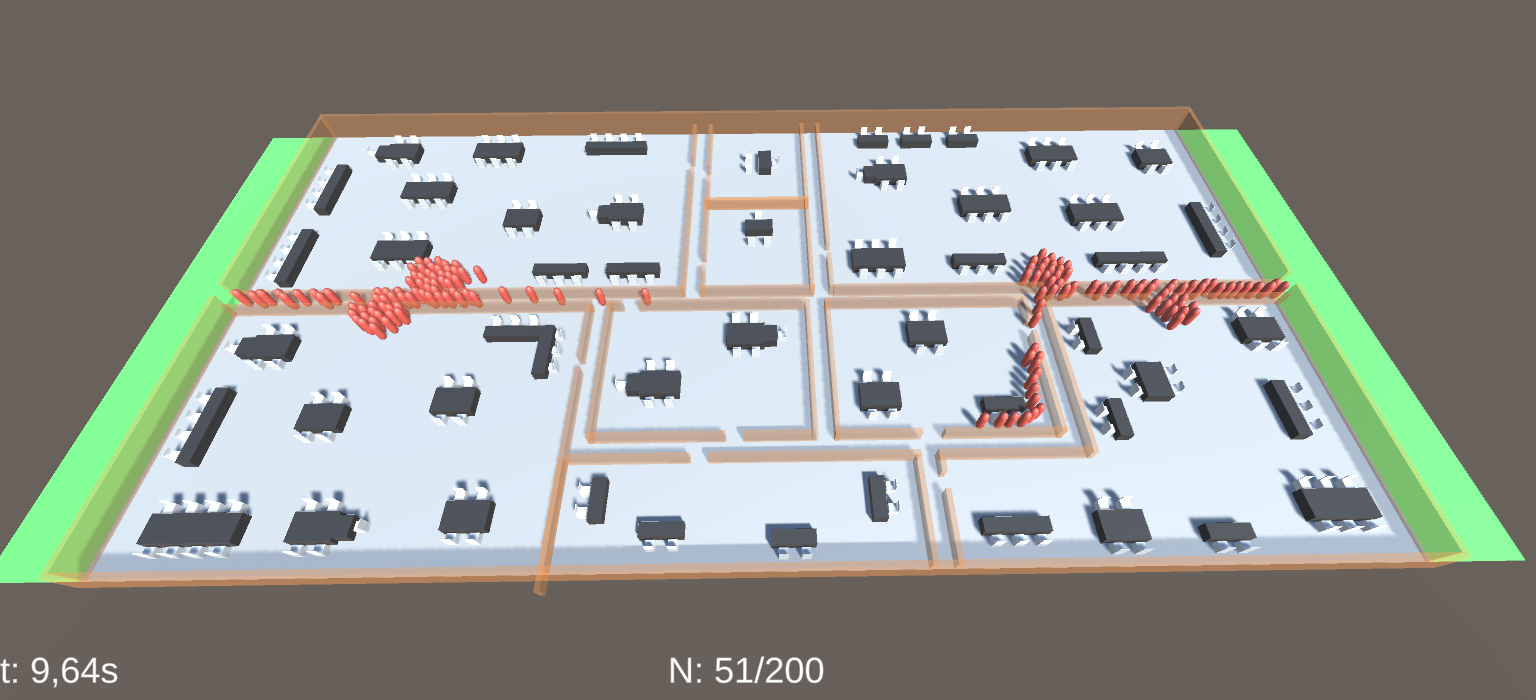
\includegraphics[scale=0.17]{1.(a) 80cm - Observations.png}\newline
\newline
$\hspace*{0.2cm}$- Parfois il n'y a que seulement une personne dans le couloir car il est trop petit (cela créée un gros ralentissement)
\newline
$\hspace*{0.2cm}$- Déjà que les gros flux ont du mal à acceder aux couloirs de base alors avec un couloir de 80cm c'est encore pire que tout 
\newline\newline

1.(a) Couloir Principal 1m :
\newline\newline
Temps moyen de dernière sortie : 24.51 s
\newline
$\hspace*{0.2cm}$- On voit qu'une fois que les personnes sont dans le couloir, il y a peu de bousculement tout le monde se dirige naturellement vers la sortie
\newline
$\hspace*{0.2cm}$- Le couloir reste par contre difficile d'accès pour les deux gros flux.
\newline\newline

1.(a) Couloir Principal 1m25 :
\newline\newline
Temps moyen de dernière sortie : 26.04 s
\newline
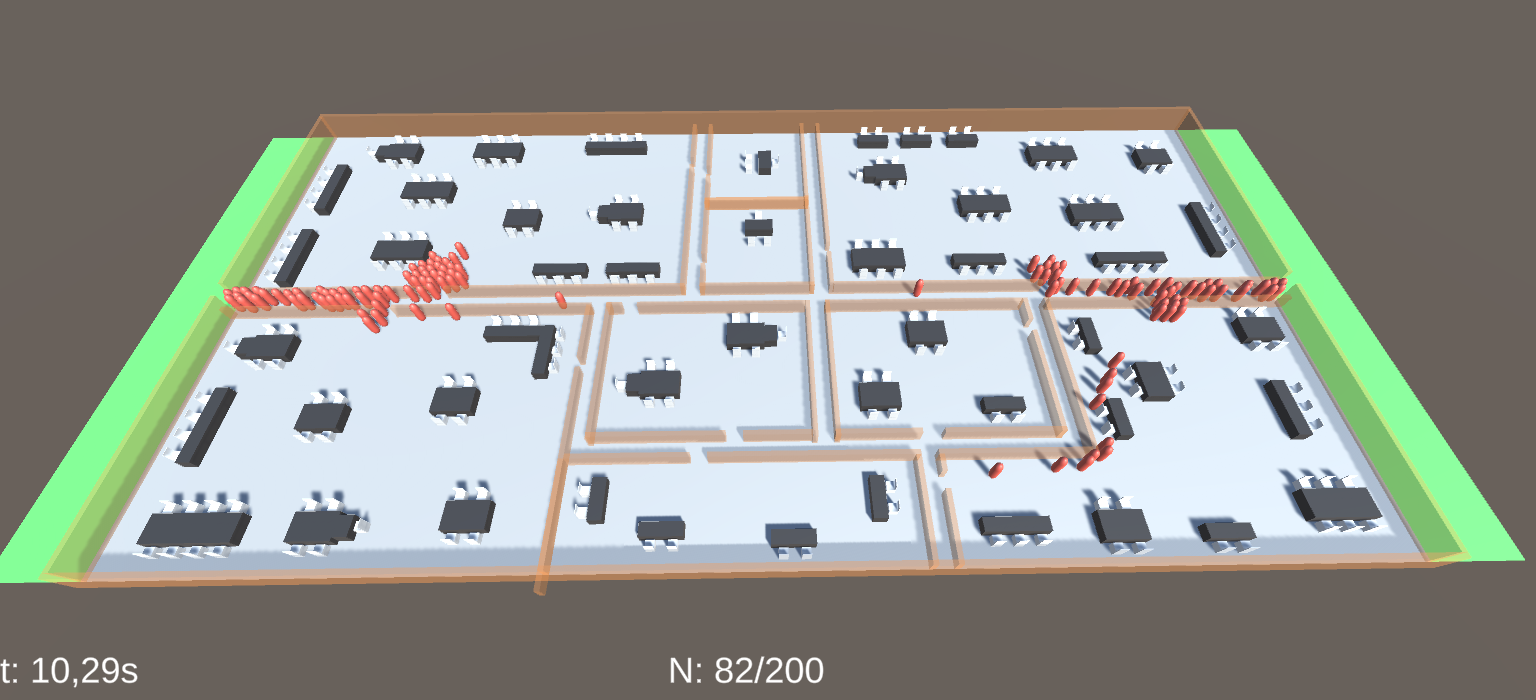
\includegraphics[scale=0.17]{1.(a) 1m25 - Observations.png}\newline
\newline
$\hspace*{0.2cm}$- La largeur du couloir permet d'accueillir maximum 2 personnes, ce qui est pareil pour la largeur des portes. Je pense que cela explique qu'il y est peu d'embouteillage au niveau des portes comparé à 1m50, ce qui est favorable
pour avoir un meilleur temps de sortie.
\newline
$\hspace*{0.2cm}$- Le fait que la largeur soit plus grande que 1m permet un peu plus de fluidité pour entrer dans ce couloir et pour que les bousculades soit moins importantes.
\newline
$\hspace*{0.2cm}$- Pourtant, 1m reste mieux que 1m25 (ceci car il y a quelque bousculade près des portes de sorties)
\newline\newline


1.(a) Couloir Principal 1m50 :
\newline\newline
Temps moyen de dernière sortie : 27.32 s
\newline
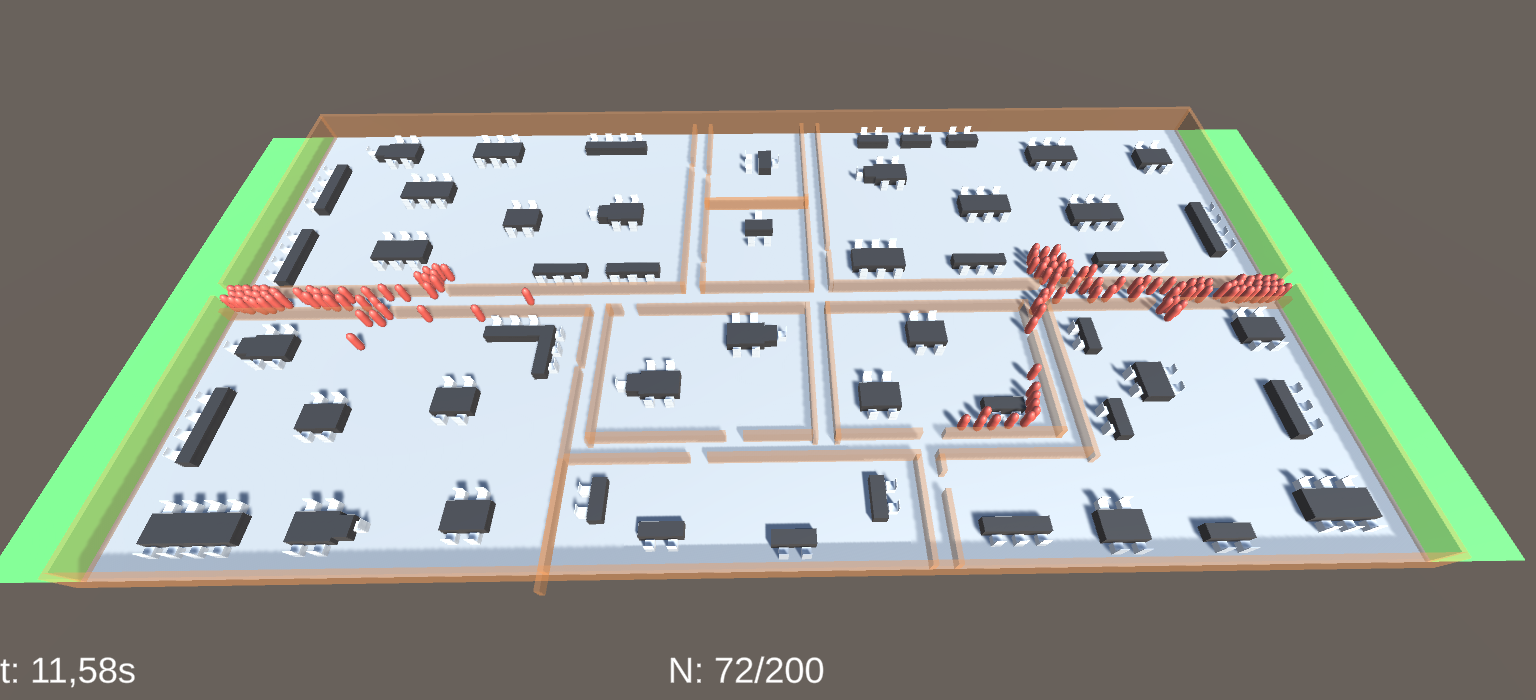
\includegraphics[scale=0.17]{1.(a) 1m5 - Problemes.png}\newline
\newline
$\hspace*{0.2cm}$- On voit que devant les portes de sortie il y a des gros flux, des blocages importants, ce qui ralentit fortement la sortie.
Donc si le couloir est trop grand par rapport aux portes, alors il y a de gros ralentissement.
\newline\newline

1.(a) Couloir Principal 2m :
\newline\newline
Temps moyen de dernière sortie : 26.26 s
\newline
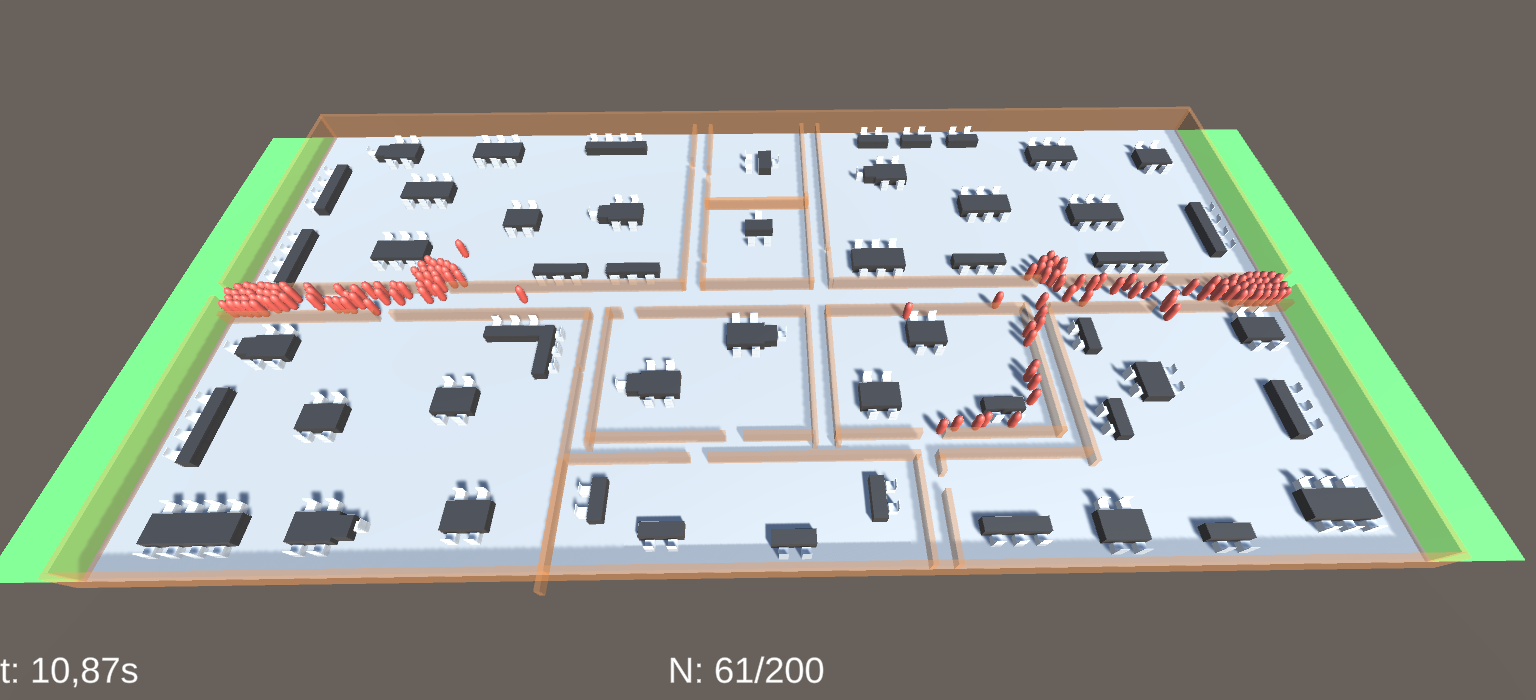
\includegraphics[scale=0.17]{1.(a) 2m - Problemes.png}\newline
\newline
$\hspace*{0.2cm}$- Le problème est encore que les personnes se bloquent devant les portes de sorties car les couloirs sont bien plus grand que les portes de sorties
donc il y a un effet entonnoir.
\newline\newline

\underline{Résultat :}
\newline
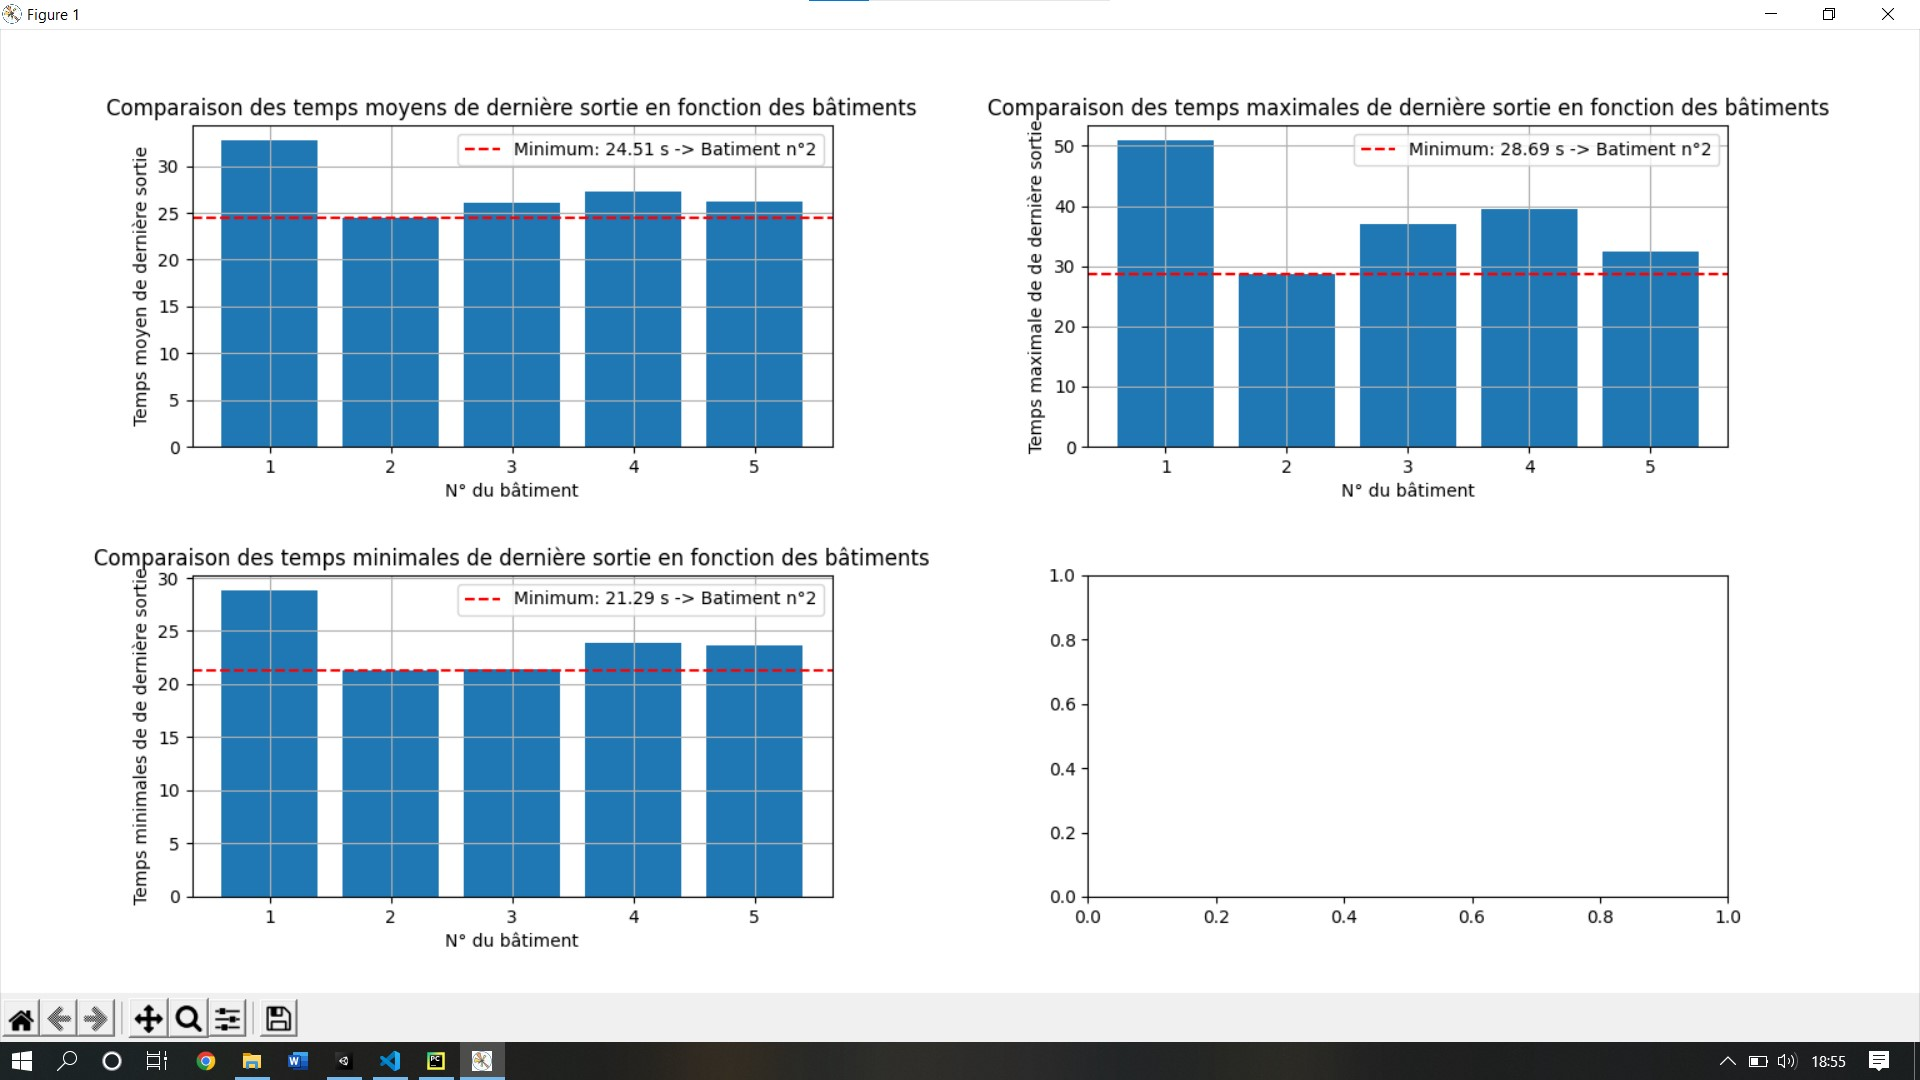
\includegraphics[scale=0.4]{1.(a) - Resultat.jpg}\newline
\newline
Les bâtiments sont numérotés par ordre croissant de taille de couloir.
\newline\newline
On peut observer qu'en effet l'hypothèse semble validé, car le meilleur temps est celui du bâtiment avec le couloir de 1m (soit la largeur des portes des sorties)
\newline
Donc cette hypothèse est à garder, elle permettra en effet d'optimiser le bâtiment final.
\newline
Ceci s'explique car avec des couloirs de la taille des portes de sortie, il n'y a aucun blocage devant ces portes de sortie. Reste à voir la taille des autres couloirs.
\end{document}